\documentclass[a4paper,12pt]{article}
\usepackage[top=2cm,left=4cm,right=4cm,bottom=2cm]{geometry}
\RequirePackage[brazil]{babel}
\usepackage[brazil]{babel}
\usepackage[utf8]{inputenc}
\usepackage{cite}
\usepackage{verbatim}
\usepackage{latexsym}
\usepackage{amsfonts}
\usepackage{amssymb}
\usepackage{graphicx}
\usepackage{hyperref}

% Title Page
\title{Transformação Data Warehouse para MapReduce no projeto ProInfoData}

\author{Tiago Rodrigo Kepe e Felipe Bolsi}


\begin{document}
\maketitle

\section{\textbf{Introdução}}

O projeto ProInfoData tem como objetivo monitorar os computadores de todas as escolas
públicas do Brasil. O monitoramento visa disponibilizar dados para que o MEC e a
sociedade acompanhem o estado de funcionamento dos computadores. Inicialmente este
parque computacional foi estimado em 500.000 computadores, atualmente, essa estimativa
aumentou para mais de 1.000.000 de máquinas, a tendência é que continue crescendo com
o tempo.
 
Para atender esta demanda o sistema foi estruturado da seguinte forma: todo computador
de escola pública brasileira terá um agente (cliente) que diariamente envia informações 
de uso e de hardware para o servidor central, além das informações do uso de rede que
foram incluídas recentemente. O servidor tem duas camadas: o WebService que recebe
informações dos agentes e as armazena no Banco de Dados (BD). Essa arquitetura pode ser
visualizada a seguir:\newline

\begin{figure}[ht]
  \centering
  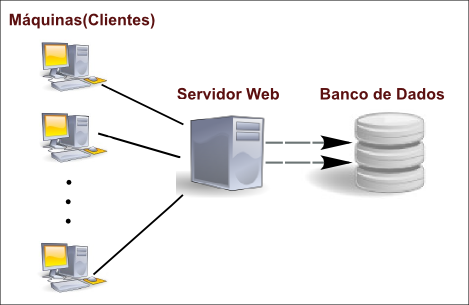
\includegraphics[width=200px,height=150px]{img/arq-bd.png}
  \caption{Visão geral da Arquitetura do ProInfoData}
\end{figure}

Como Sistema de Gerenciamento de Banco de Dados foi escolhido PostgreSQL, um dos 
motivos dessa escolha é por que o PostgreSQL é um software livre, entretanto,
para comportar o volume de dados gerado foi necessário desenvolver uma arquitetura de
armazenamento robusta e escalável. A arquitetura proposta foi baseada em armazém de
dados Data Warehouse (DW) que é direcionada às operações de leitura, favorecendo a 
análise de grandes volumes de dados e a geração de relatórios complexos, entraremos em
mais detalhes no capítulo 2.

No entanto, com o aumento emergente do número de máquinas e com o acréscimo das
informações do uso de rede, o volume de dados tornou-se extremamente grande, fato que 
nos levou a propor um nova solução para o armazenamento dos dados e para realização
das consultas disponíveis no \href {http://seed.c3sl.ufpr.br/seed/attendance/index.html}
{portal do projeto}.

Nossa proposta baseia-se em uma tecnologia emergente, chamada MapReduce. Essa solução 
mostrou-se eficiente em diversas implementações, a mais conhecida é o sistema de 
armazenamento e busca do Google, ver \cite{MapReduceGoogle} ou
\href {http://labs.google.com/papers/mapreduce.html} {artigo MapReduce Google}.

Acreditamos que o grande desafio dessa solução será a transformação do modelo baseado 
em Data Warehouse para um modelo MapReduce.

No capítulo 2 descrevemos com mais detalhes o conceito de Data Warehouse e a arquitetura
do projeto ProInfoData. No capítulo 3 descrevemos o conceito de MapReduce, as 
tecnoligias que serão utilizadas Hive e Hadoopt e porque utlizar MapReduce no 
ProInfoData. No capítulo 4 deparamos com nosso grande desafio em propor um método de 
transformação de Data Warehouse para MapReduce. Enfim, no capítulo 5 chegamos as
conclusões dessa monografia.

\section{\textbf{Data Warehouse}}

Segundo Silberschatz e Korth \cite{Silber} "As consultas ao banco de dados
normalmente são projetadas para extrair informações específicas, como saldo
de um conta ou a soma dos saldos de conta de um cliente. Porém, consultas
projetadas para ajudar a formular um estratégia corporativa normalmente
exigem a agregação em um escala muito maior e incluem análise estatística
não expressa facilmente com os recursos da SQL que já vimos anteriormente.
Essas cosultas normalmente precisam acessar dados vindos de várias origens.

%Normalmente as consultas em banco de dados são arquitetadas para extrair
%informações específicas. Porém, consultas projetadas para extrair
%informações estratégicas para tomada de decisão, normalmente, exigem a
%agregação numa escala bem maior e incluem fatores estatísticos complexos que
%não são expressados facilmente com os recursos da SQL, pois normalmente
%essas consultas precisam acessar dados oriundos de várias fontes.

Um depósito de dados(data warehouse) é um repositório de dados oriundos de
várias fontes e armazenados sob um banco de dados comum, unificado. Os
dados armazenados no depósito são submetidos a análises e agregações
complexas. Também é possível utilizar técnicas para descobrir regras e
padrões a partir dos dados, facilitando, assim, a tomada de decisão.

Os dados procedentes do depósito podem ser explorados pelas empresas para
ajudar com o suporte à decisão. Essas informações são de alto nível obtidas a partir de dados detalhados armazenados no depósito.

Existem várias técnicas para 

2 - Explicar o que é Data Mart 

3 - Descrever a arquitetura do BD no ProInfoData como abaixo e colocar umas figuras

A arquitetura possui três etapas: carregamento, armazenamento e leitura de dados.
O carregamento consiste em receber e consolidar os dados no DW, o armazenamento é o
próprio histórico de dados do DW e a etapa de leitura organiza os dados para otimizar 
as consultas. Essas etapas são implementadas em três componentes: staging area,
DW e Data Marts (DM).


A staging area é responsável por receber os dados dos clientes sem nenhuma manipulação, 
esses dados são armazenados temporariamente neste componente. Após o carregamento da 
staging area, os dados são extraídos, transformados e consolidados no DW. Finalmente os
dados são sumarizados no DM que foi projetado para otimizar as consultas. Em todos 
esses componentes foram realizados testes de desempenho, utilizando uma metodologia 
baseada em um modelo incremental de hardware e software. O objetivo é avaliar o sistema
 partindo de um ambiente menos complexo para o mais complexo, usando cargas
 intermediárias até o ponto limite do sistema. Com isso, além de encontrar a carga 
máxima que o sistema suporta, fornece também resultados parciais que facilitam a
 avaliação de estresse de hardware.  Os testes de escrita no BD mostraram que a 
arquitetura proposta chega a atender 334 transações por segundo. Já os testes de 
consulta alcançou o número de 142 transações por segundo. Com estes resultados, a
 arquitetura mostrou-se eficiente, atendendo as conexões e o volume de dados esperado.

\section{\textbf{MapReduce}}
1 - Explicar conceito

2 - Explicar o que é Hadoop e Hive (talvez criar uma subseção)

\section{\textbf{Transformação}}
1 - Como fazer

2 - Como ficarm os Data Marts, se eles serão necessários

3 - Exemplos como ficaria do ProInfoData

\section{\textbf{Conclusão}}
1 - é viável, fácil...

\bibliographystyle{plain}
\bibliography{tg}
\end{document}
